This chapter covers the basic theory and main solution methods for
stationary MDPs over an infinite horizon, with the discounted return
criterion, which we will refer to as \textit{discounted MDPs}. 
% In this case, we will show that stationary policies are optimal.

The discounted return problem is the most ``well behaved'' among all
infinite horizon problems (such as average return and stochastic
shortest path), and its theory is relatively simple, both in
the planning and the learning contexts. For that reason, as well as
its usefulness, we will consider here the discounted problem and its
solution in some detail.

%Contents:
%5.1 Problem Statement
%5.2 Preliminaries: The Fixed-policy Value Function
%5.3 Overview: Main Algorithms
%5.4 Contraction Operators
%5.5 Proof of Bellman's Optimality Equation
%5.6 Value Iteration
%5.7 Policy Iteration
%5.8 Some variants on Value and Policy Iteration
%5.9 Linear Programming Solutions

\section{Problem Statement} \label{sec:inf_horizon_prob}

We consider a stationary (time-invariant) MDP, with a finite state
space $\States$, finite action set $\Actions$, a fixed reward function $r(s,a)$, and a fixed transition kernel
$\transitionkernel = \{\transitionprob(\state'|\state,\action)\}$ over  the infinite time horizon
${\T} = \{ 0,1,2, \ldots \} $.

Our goal is to maximize the expected discounted return, which is
defined for each control policy $\policy $ and initial state
${\state_0} = \state$ as follows:
\begin{align*}
\Value_\discount ^\policy (\state) &= {\E^\policy }\left(\left. \sum\limits_{\ttime = 0}^\infty  {{\discount ^\ttime}\reward({\state_\ttime},{\action_\ttime})} \right|{\state_0} = \state\right)\\
 &\equiv {\E^{\policy ,\state}}\left(\sum\limits_{\ttime = 0}^\infty  {{\discount ^\ttime}\reward({\state_\ttime},{\action_\ttime})} \right),
\end{align*}
where $\E^{\policy ,\state}$ uses the distribution induced by policy
$\policy$ starting at state $\state$. Here,
\begin{itemize}
  \item $\reward : \States \times \Actions \to \mathbb R$ is the (running, immediate, or instantaneous) expected reward function, i.e., $\reward(\state,\action)=\E[R|\state,\action]$.
  \item $\discount  \in (0,1)$ is the discount factor.
\end{itemize}

We observe that $\discount  < 1$  ensures convergence of the
infinite sum (since the rewards
$\reward({\state_\ttime},{\action_\ttime})$ are uniformly bounded because $\States$ and $\Actions$ are finite).
With $\discount  = 1$ we obtain the total return criterion, which is
harder to handle due to possible divergence of the sum.

Let $\Value_\discount ^*(\state)$ denote the maximal expected value
of the discounted return, over all (possibly history dependent and
randomized) control policies, i.e.,
\[\Value_\discount ^*(\state) = \mathop {\sup }\limits_{\policy  \in {\Pi _{HS}}} \Value_\discount ^\policy (\state).\]


Our goal is to find an optimal control policy ${\policy ^*}$ that
attains that maximum (for all initial states), and compute the
numeric value of the optimal return $\Value_\discount ^*(\state)$.
As we shall see, for this problem there always exists an optimal
deterministic stationary policy.

\begin{remark}
    As usual, the discounted performance criterion can be defined in terms of cost:
\[\Cost_\discount ^\policy (\state) = {\E^{\policy ,\state}}(\sum\limits_{\ttime = 0}^\infty  {{\discount ^\ttime}\cost({\state_\ttime},{\action_\ttime})} )\;,\]
where $\cost(\state,\action)$ is the running cost function. Our goal
is then to minimize the discounted cost $\Cost_\discount ^\policy
(\state)$. Since minimizing cost and maximizing reward are equivalent, we will focus on maximizing rewards throughout the book.
\end{remark}


\section{The Fixed-Policy Value Function}\label{s:FP_VF}

We start the analysis by defining and computing the value function for a fixed stationary policy. This intermediate step is required for later analysis of our optimization problem,  and also serves as a gentle introduction to the value iteration approach.

For a stationary policy $\policy :\States \to \Actions$, we define
the value function $\Value_\discount^\policy (\state),\;\state \in \States$
simply as the corresponding discounted return:
\[\Value_{\discount}^\policy (\state) \buildrel \Delta \over = {\E^{\policy ,\state}}\left(\sum\limits_{\ttime = 0}^\infty  {{\discount ^\ttime}\reward({\state_\ttime},{\action_\ttime})} \right),   \quad \forall \state \in  \States\].
To reduce clutter we will omit the $\discount$ subscript in the following and abbreviate 
$\Value_{\discount}^\policy (\state)$ as $\Value^\policy (\state)$
\begin{lemma}\label{lem:FP_Bellman}
For $\policy\in\Pi_{SD}$, the value function $\Value_{}^\policy $
satisfies the following set of $|\States|$ linear equations:
\begin{equation}\label{eq:FP_Bellman}
{\Value^\policy }{\kern 1pt} (\state) = \reward(\state,\policy
(\state)) + \discount \sum_{\state' \in \States} \transitionprob(\state' | \state, \policy(\state)) \Value^{\policy} (\state'), \qquad \forall \state \in \States.
\end{equation}
\end{lemma}


\begin{proof} We first note that
\begin{align*}
\Value_{}^\policy (\state) &\buildrel \Delta \over = {\E^\policy }(\sum\limits_{\ttime = 0}^\infty  {{\discount ^\ttime}\reward({\state_\ttime},{\action_\ttime})} |{\state_0} = \state)\\
 &= {\E^\policy }(\sum\limits_{\ttime = 1}^\infty  {{\discount ^{t - 1}}\reward({\state_\ttime},{\action_\ttime})} |{\state_1} = \state),
\end{align*}
since both the model and the policy are stationary and in particular time invariant. Now,
\begin{align*}
\Value_{}^\policy (\state) &= \reward(\state,\policy (\state)) + {\E^\policy }(\sum\limits_{\ttime = 1}^\infty  {{\discount ^\ttime}\reward({\state_\ttime},\policy ({\state_\ttime}))} |{\state_0} = \state)\\
&= \reward(\state,\policy (\state)) + {\E^\policy }\left[\left.{\E^\policy }\left(\sum\limits_{\ttime = 1}^\infty  {{\discount ^\ttime}\reward({\state_\ttime},\policy ({\state_\ttime}))} |{\state_0} = \state, \state_1=\state'\right)\right|{\state_0} = s\right]\\
 &= \reward(\state,\policy (\state)) + \sum\limits_{\state' \in \States}^{} {\transitionprob(\state'|\state,\,} \policy (\state)){\E^\policy }(\sum\limits_{\ttime = 1}^\infty  {{\discount ^\ttime}\reward({\state_\ttime},\policy ({\state_\ttime}))} |{\state_1} = \state')\\
 &= \reward(\state,\policy (\state)) + \discount \sum\limits_{\state' \in \States}^{} {\transitionprob(\state'|\state,\,} \policy (\state)){\E^\policy }(\sum\limits_{\ttime = 1}^\infty  {{\discount ^{t - 1}}\reward({\state_\ttime},{\action_\ttime})} |{\state_1} = \state')\\
 &= \reward(\state,\policy (\state)) + \discount \sum\limits_{\state' \in \States}^{} {\transitionprob(\state'|\state,\,} \policy (\state)){\Value^\policy }(\state').
\end{align*}
The first equality is by the definition of the value function. The
second equality follows from the law of total expectation,
conditioning $\state_1 = \state'$ and taking the expectation over
it. By definition ${\action_\ttime} = \policy ({\state_\ttime})$.
The third equality follows similarly to the finite-horizon case
(Lemma \ref{lem:finite_horizon_VI}, in Chapter~\ref{chapter:MDP-FH}).
The fourth is simple algebra, taking one multiple of the discount
factor $\discount$ outside. The last, by the observation in the
beginning of the proof.
\end{proof}

We can write the linear equations in \eqref{eq:FP_Bellman} in vector
form as follows. Define the column vector ${\reward^\policy } =
{({\reward^\policy }(\state))_{\state \in \States}}$ with components
${\reward^\policy }(\state) = \reward(\state,\policy (\state))$, and the
transition matrix ${\transitionkernel^\policy }$ with components ${\transitionkernel^\policy
}(\state'|\state) = \transitionprob(\state'|\state,\policy (\state))$. Finally,
let ${\Value^\policy }$ denote a column vector with components
${\Value^\policy }(\state)$. Then \eqref{eq:FP_Bellman} is
equivalent to the linear equation set
\begin{equation}\label{eq:PF_Bellman_vector}
{\Value^\policy } = {\reward^\policy } + \discount {\transitionkernel^\policy
}{\Value^\policy }.
\end{equation}

\begin{lemma}\label{lem:FP_Bellman_sol}
For any policy $\pi \in \Pi_{SD}$ 
the set of linear equations \eqref{eq:FP_Bellman} or
\eqref{eq:PF_Bellman_vector}, with ${\Value^\policy }$ as variables,
has a unique solution ${\Value^\policy }$, which is given by
\[{\Value^\policy } = {(I - \discount {\transitionkernel^\policy })^{ -
1}}{\reward^\policy }.\]
\end{lemma}
\begin{proof}
We only need to show that the square matrix $I - \discount
{\transitionkernel^\policy }$ is non-singular.  Let $({\lambda _i})$ denote the
eigenvalues of the matrix ${\transitionkernel^\policy }$. Since ${\transitionkernel^\policy }$ is a
stochastic matrix (row sums are 1), then $|{\lambda _i}| \le 1$ (see the proof of Theorem~\ref{Thm:MC-stationary}).
Now, the eignevalues of $I - \discount {\transitionkernel^\policy }$ are $(1 -
\discount {\lambda _i})$, and satisfy $|1 - \discount {\lambda _i}|
\ge 1 - \discount  > 0$.
\end{proof}

Combining Lemma \ref{lem:FP_Bellman} and Lemma \ref{eq:PF_Bellman_vector}, we obtain the following.

\begin{proposition}\label{prop:FP_Bellman}
For any $\pi\in \Pi_{SD}$. The value function ${\Value^\policy } =
[{\Value^\policy }(\state)]$ is the unique solution of Equation
\eqref{eq:PF_Bellman_vector}, and is given by \[{\Value^\policy } = {(I -
\discount {\transitionkernel^\policy })^{ - 1}}{\reward^\policy }.\]
\end{proposition}

Proposition \ref{prop:FP_Bellman} provides a closed-form formula for
computing $\Value_{}^\policy$. However, for large systems, computing
the inverse ${(I - \discount {\transitionkernel^\policy })^{ - 1}}$ may be
computationally expensive. In that case, the following value
iteration algorithm provides an alternative, iterative method for
computing $\Value_{}^\policy$.

% \begin{algorithm_}\textbf{Fixed-policy value iteration}
% \begin{enumerate}
%   \item Let ${\Value_0} = {({\Value_0}(\state))_{\state \in \States}}$ be arbitrary.
%   \item For $n = 0,1,2, \ldots $, set
% \[\Value_{n + 1}^{}{\kern 1pt} (\state) = \reward(\state,\policy (\state)) + \discount \sum\nolimits_{\state' \in \States} {\transitionprob(\state'|\state,\policy (\state))\Value_n^{}{\kern 1pt} (\state')} \;,\quad \;\forall \state \in \States\]
% \tab{or, equivalently,}
% \[{\Value_{n + 1}} = {\reward^\policy } + \discount {\transitionkernel^\policy }{\Value_n}.\]
% \end{enumerate}
% \end{algorithm_}

\begin{algorithm}
\caption{Fixed-policy Value Iteration}
\label{alg:fixed_policy_VI}
\begin{algorithmic}[1]
\State \textbf{Initialization:} Set $\Value_0 = (\Value_0(\state))_{\state \in \States}$ arbitrarily.
\State \textbf{For} {$n = 0, 1, 2, \ldots$}
    \State \label{alg:fixed_policy_VI:line3} \quad Set $\Value_{n + 1}(\state) = \reward(\state, \policy(\state)) + \discount \sum_{\state' \in \States} \transitionprob(\state'|\state, \policy(\state)) \Value_n(\state') \quad \forall \state \in \States$
    % \State Or, equivalently,
    % \State $\Value_{n + 1} = \reward^\policy + \discount \transitionkernel^\policy \Value_n$.
\end{algorithmic}
\end{algorithm}

Note that Line \ref{alg:fixed_policy_VI:line3} in Algorithm \ref{alg:fixed_policy_VI} can equivalently be written in matrix form as:
\begin{equation*}
    \Value_{n + 1} = \reward^\policy + \discount \transitionkernel^\policy \Value_n.
\end{equation*}

%Then \[{\Value_n} \to \Value_{}^\policy \]component-wise, that is,
%\[{\lim _{n \to \infty }}{\Value_n}(\state) = \Value_{}^\policy (\state),\quad \;\state \in \States\]

\begin{proposition}[\textbf{Convergence of fixed-policy value iteration}]\label{prop:FP_VI}
We have that ${\Value_n} \to \Value_{}^\policy$ component-wise, that is,
\[{\lim _{n \to \infty }}{\Value_n}(\state) = \Value_{}^\policy (\state),\quad \;\forall \state \in \States.\]
\end{proposition}
\begin{proof}
Note that,
\begin{align*}
{\Value_1}{\kern 1pt} (\state) &= \reward(\state,\policy (\state)) + \discount \sum\nolimits_{\state' \in \States} {\transitionprob(\state'|\state,\policy (\state))\Value_0^{}{\kern 1pt} (\state')} \;\\
 &= {\E^\policy }(\reward({\state_0},{\action_0}) + \discount {\Value_0}({\state_1})|{\state_0} = \state).
\end{align*}
Continuing similarly, we obtain that
\[{\Value_n}{\kern 1pt} (\state) = {\E^\policy }(\sum\limits_{\ttime = 0}^{n - 1} {{\discount ^\ttime}\reward({\state_\ttime},{\action_\ttime})}  + {\discount ^n}{\Value_0}({s_n})|{\state_0} = \state).\]
Note that ${\Value_n}{\kern 1pt} (\state)$ is the $n$-stage
discounted return, with terminal reward ${\reward_n}({\state_n}) =
{\Value_0}({\state_n})$. Comparing with the definition of
$\Value_{}^\policy $, we can see that
\[{\Value^\policy }(\state) - {\Value_n}{\kern 1pt} (\state) = {\E^\policy }(\sum\limits_{\ttime = n}^\infty  {{\discount ^\ttime}\reward({\state_\ttime},{\action_\ttime})}  - {\discount ^n}{\Value_0}({\state_n})|{\state_0} = \state).\]
Denoting $\Rmax = {\max
_{\state,\action}}|\reward(\state,\action)|$, ${\bar \Value_0} =
{\max _s}|\Value_0(\state)|$ we obtain
\[|{\Value^\policy }(\state) - {\Value_n}{\kern 1pt} (\state)| \le {\discount ^n}(\frac{{\Rmax}}{{1 - \discount }} + {\bar \Value_0})\]
which converges to 0 since $\discount  < 1$.
\end{proof}

\paragraph{Comments:}
\begin{itemize}
  \item The proof provides an explicit bound on $|{\Value^\policy }(\state) - {\Value_n}{\kern 1pt} (\state)|$. It may be seen that the convergence is exponential, with rate $O({\discount ^n})$.
  \item Using vector notation, it may be seen that
          \[{\Value_n}{\kern 1pt}  = {\reward^\policy } + \discount{\transitionkernel^\policy }{\reward^\policy } +  \ldots  + {(\discount{\transitionkernel^\policy })^{n - 1}}{\reward^\policy } + {(\discount{\transitionkernel^\policy })^n}{\Value_0} = \sum\limits_{\ttime = 0}^{n - 1} {{{(\discount{\transitionkernel^\policy })}^\ttime}{\reward^\policy }}  + {(\discount{\transitionkernel^\policy })^n}{\Value_0}.\]
Similarly,    ${\Value^\policy } = \sum\limits_{\ttime = 0}^\infty
{{{(\discount{\transitionkernel^\policy })}^\ttime}{\reward^\policy }}$.
\end{itemize}

\paragraph{In summary:}
\begin{itemize}
  \item Proposition \ref{prop:FP_Bellman} allows to compute $\Value_{}^\policy $ by solving a set of $|\States|$ linear equations.
  \item Proposition \ref{prop:FP_VI} computes $\Value_{}^\policy $ by an infinite recursion, that converges exponentially fast.
\end{itemize}

\section{Overview: The Main DP Algorithms}

We now return to the optimal planning problem formulated in Section
\ref{sec:inf_horizon_prob}. Recall that  $\Value_\discount
^*(\state) = {\sup _{\policy  \in \Pi }}_{_{HS}}\Value_\discount
^\policy (\state)$ is the optimal discounted return. We further
denote
\[{\Value^*}(\state) \buildrel \Delta \over = \Value_\discount ^*(\state),    \quad  \forall \state \in \States,\]
and refer to ${\Value^*}$ as the optimal value function. Depending
on the context, we consider ${\Value^*}$ either as a function
$\Value^* : \States \to \mathbb R$, or as a column vector
${\Value^*} = {[\Value(\state)]_{\state \in \States}}$.

The following optimality equation provides an explicit
characterization of the value function, and shows that an optimal
stationary policy can easily be computed if the value function is
known. (See the proof in Section~\ref{sec:Bellman-Opt}.)

\begin{theorem}[\textbf{Bellman's Optimality Equation}]\label{thm:inf_Bellman} The following statements hold:
\begin{enumerate}
  \item $\Value_{}^*$ is the unique solution of the following set of (nonlinear) equations:
\begin{equation}\label{eq:Bellman}
\Value(\state) = \mathop {\max }\limits_{\action \in \Actions}
\left\{ {\reward(\state,\action) + \discount \sum\nolimits_{\state'
\in \States} {\transitionprob(\state'|\state,\action)\Value(\state')} } \right\},
\quad \forall \state \in \States.
\end{equation}
  \item Any stationary policy ${\policy ^*}$ that satisfies
\[{\policy ^*}(\state) \in \arg {\max _{\action \in \Actions}}\left\{ {\reward(\state,\action) + \discount \sum\nolimits_{\state' \in \States} {\transitionprob(\state'|\state,\action)\Value(\state')} } \right\} \quad \forall \state \in \States, \]
     is an optimal policy (for any initial state ${\state_0} \in \States$).
\end{enumerate}
\end{theorem}
The optimality equation \eqref{eq:Bellman} is non-linear, and
generally requires iterative algorithms for its solution. The main
iterative algorithms are \textbf{value iteration} and \textbf{policy
iteration}. In the following we provide the algorithms and the basic
claims. Later in this chapter we formally prove the results
regarding value iteration (Section~\ref{sec:VI}) and policy
iteration (Section~\ref{sec:PI}).


% \begin{algorithm_}\textbf{Value Iteration (VI)}\label{alg:VI}
% \begin{enumerate}
%   \item Let ${\Value_0} = {({\Value_0}(\state))_{\state \in \States}}$ be arbitrary.
%   \item For $n = 0,1,2, \ldots $, set
% \[{\Value_{n + 1}}(\state) = \mathop {\max }\limits_{\action \in \Actions} \left\{ {\reward(\state,\action) + \discount \sum\nolimits_{\state' \in \States} {\transitionprob(\state'|\state,\action){\Value_n}(\state')} } \right\},    \quad \forall \state \in \States\]
% \end{enumerate}
% \end{algorithm_}

\begin{algorithm}
\caption{Value Iteration (VI)}
\label{alg:VI}
\begin{algorithmic}[1]
\State \textbf{Initialization:} Set $\Value_0 = (\Value_0(\state))_{\state \in \States}$ arbitrarily.
\State \textbf{For} {$n = 0, 1, 2, \ldots$}
    \State \quad Set $\Value_{n + 1}(\state) = \max_{\action \in \Actions} \left\{ \reward(\state,\action) + \discount \sum_{\state' \in \States} \transitionprob(\state'|\state,\action)\Value_n(\state') \right\}, \quad \forall \state \in \States$
\end{algorithmic}
\end{algorithm}



\begin{theorem}[\textbf{Convergence of value iteration}]\label{thm:_VI}
We have ${\lim _{n \to \infty }}{\Value_n} = \Value_{}^*$
(component-wise). The rate of convergence is exponential, at rate
$O({\discount ^n})$.
\end{theorem}

\begin{proof}
%[\textbf{Proof of Theorem \ref{thm:_VI}:}]
Using our previous results on value iteration for the finite-horizon
problem, namely the proof of Proposition~\ref{prop:FP_VI}, it
follows that
\[{\Value_n}(\state) = \mathop {\max }\limits_\policy  {\E^{\policy ,\state}}(\sum\limits_{\ttime = 0}^{n - 1} {{\discount ^\ttime}{R_t} + } {\discount ^n}{\Value_0}({\state_n})).\]
Comparing to the optimal value function
\[{\Value^*}(\state) = \mathop {\max }\limits_\policy  {\E^{\policy ,\state}}(\sum\limits_{\ttime = 0}^\infty  {{\discount ^\ttime}{R_t}} ),\]
it may be seen that that
                                \[|{\Value_n}(\state) - \Value_{}^*(\state)| \le {\discount ^n}(\frac{{\Rmax}}{{1 - \discount }} + ||{\Value_0}|{|_\infty }).\]
As $\discount  < 1$, this implies that ${\Value_n}$ converges to
$\Value_\discount ^*$  exponentially fast.
\end{proof}

The value iteration algorithm iterates over the value functions, with asymptotic convergence. The policy iteration algorithm iterates over stationary policies, with each new policy better than the previous one. This algorithm converges to the optimal policy in a finite number of steps.

% \begin{algorithm_}\textbf{Policy Iteration (PI)}\label{alg:PI}
% \begin{enumerate}
% \item Initialization: choose some stationary policy ${\policy _0}$.
% \item For $k = 0,1, \ldots $:
% \begin{enumerate}
% \item Policy evaluation: compute ${\Value^{{\policy _k}}}$.\\
%      %\coderemark{}
%      (For example, use the explicit formula  ${\Value^{{\policy _k}}} = {(I - \discount {\transitionkernel^{{\policy _k}}})^{ - 1}}{\reward^{{\policy
%      _k}}}$.)
% \item Policy Improvement: Compute ${\policy _{k + 1}}$, a greedy policy with respect to ${\Value^{{\policy _k}}}$:
% \[{\policy _{k + 1}}(\state) \in \arg {\max _{\action \in \Actions}}\left\{ {\reward(\state,\action) + \discount \sum\nolimits_{\state' \in \States} {\transitionprob(\state'|\state,\action){\Value^{{\policy _k}}}(\state')} } \right\},\quad \forall \state \in \States.\]
% \item Stop if $\policy _{k + 1} = \policy _k$
% %${\Value^{{\policy _{k + 1}}}} = {\Value^{{\policy _k}}}$
% (or if ${\Value^{{\policy _k}}}$ satisfied the optimality equation), else
% continue.
% %\footnote{YM: note that we compute the value of $k+1$ only in the next iteration }
% \end{enumerate}
% \end{enumerate}
% \end{algorithm_}

\begin{algorithm}
\caption{Policy Iteration (PI)}
\label{alg:PI}
\begin{algorithmic}[1]
\State \textbf{Initialization:} choose some stationary policy $\policy_0$.
\State \textbf{For} {$k = 0, 1, 2,\ldots$}
    \State \quad \textbf{Policy Evaluation:} Compute $\Value^{\policy_k}$.
    \State \quad \quad (For example, use the explicit formula $\Value^{\policy_k} = (I - \discount \transitionkernel^{\policy_k})^{-1}\reward^{\policy_k}$)
    \State \quad \textbf{Policy Improvement:} Compute $\policy_{k+1}$, a greedy policy with respect to $\Value^{\policy_k}$:
    \State \quad $\policy_{k+1}(\state) \in \arg \max_{\action \in \Actions} \left\{ \reward(\state,\action) + \discount \sum_{\state' \in \States} \transitionprob(\state'|\state,\action)\Value^{\policy_k}(\state') \right\}, \forall \state \in \States.$
    \State \quad \textbf{If} $\policy_{k+1} = \policy_k$ (or if $\Value^{\policy_k}$ satisfies the optimality equation)
    \State \quad \quad \textbf{Stop}
\end{algorithmic}
\end{algorithm}

\begin{theorem}[\textbf{Convergence of policy iteration}]\label{thm:_PI}
The following statements hold:
\begin{enumerate}
  \item Each policy ${\policy _{k + 1}}$ is improving over the previous one ${\policy _k}$, in the sense that ${\Value^{{\policy _{k + 1}}}} \ge {\Value^{{\policy _k}}}$ (component-wise).
  \item ${\Value^{{\policy _{k + 1}}}} = {\Value^{{\policy _k}}}$ if and only if ${\policy _k}$ is an optimal policy.
  \item Consequently, since the number of stationary deterministic policies is finite, ${\policy _k}$ converges to the optimal policy after a finite number of steps.
\end{enumerate}
\end{theorem}

\begin{remark}
An additional solution method for DP planning relies on a Linear
Programming formulation of the problem. See chapter~\ref{chapter-LP}.
\end{remark}
%A Linear Program (LP) is
%simply an optimization problem with linear objective function and linear constraints.
% We will provide additional details later in this Chapter, in Section~\ref{chapter-discount:section:LP}.

\section{Contraction Operators}

The basic proof methods of the DP results mentioned above rely on
the concept of a \emph{contraction operator}. We provide here the
relevant mathematical background, and illustrate the contraction
properties of some basic Dynamic Programming operators.

\subsection{The contraction property}
Recall that a norm $|| \cdot ||$ over $\reals^n$  is a real-valued
function $\|\cdot\| : \reals^d \to \mathbb R^+$ such that, for any
pair of vectors $x,y \in \reals^d$  and scalar $a\in\reals$,
\begin{enumerate}
  \item $||ax|| = |a| \cdot ||x||$,
  \item $||x + y|| \le ||x|| + ||y||$,
  \item $||x|| = 0$ only if $x = 0$.
\end{enumerate}

Common examples are the p-norm $||x|{|_p} = (\sum\nolimits_{i = 1}^d
{{{|{x_i}|}^p}{)^{1/p}}} $ for $p \ge 1$, and in particular the
Euclidean norm ($p = 2$). Here we will mostly use the max-norm:
\[||x|{|_\infty } = {\max _{1 \le i \le d}}|{x_i}|.\]
Unless otherwise mentioned, we will omit the $\infty$ and use $\|\cdot\| $ to abbreviate the max-norm throughout the book.

Let $T:\mathbb R^d \to \mathbb R^d$  be a vector-valued function
over $\mathbb R^d$   ($d \ge 1$).
%\footnote{YM: Maybe use another
%letter. We have T for the horizon how about $\operator$.
%Need to define a Macro for it.
%}
%
We equip $\mathbb R^d$ with some norm $||
\cdot ||$, and refer to $T$ as an \emph{operator } over $\mathbb
R^d$. Thus, $T(v) \in \mathbb R^d$ for any $v \in \mathbb R^d$. We
also denote ${T^n}(v) = T({T^{n - 1}}(v))$ for  $n \ge 2$. For
example, ${T^2}(v) = T(T(v))$.

\begin{definition} The operator $T$ is called a contraction operator with respect to a norm $\|\cdot \|$, if there exists $\beta  \in (0,1)$ (the contraction coefficient) such that
                            \[||T({v_1}) - T({v_2})|| \le \beta ||{v_1} - {v_2}||,\]
                            for all $v_1,v_2 \in \mathbb R^d$. In which case,  $T$ is called a $\beta$-contraction operator.
\end{definition}
When the norm is clear from the context, we will omit explicit mentioning of it.

\subsection{The Banach Fixed Point Theorem}
The following celebrated result applies to contraction operators. While we quote the result for $\mathbb R^d$, we note that it applies in much greater generality to any Banach space (a complete normed space), with essentially the same proof.

\begin{theorem}[\textbf{Banach's fixed point theorem}]
\label{chapter-discount:thm:Banach}
 Let $T:\mathbb R^d \to \mathbb R^d$  be a
contraction operator with respect to some norm $\|\cdot \|$. Then
\begin{enumerate}
  \item The equation $T(v) = v$ has a unique solution  $\Value^*\in \mathbb R^d$.
  \item For any $v_0 \in \mathbb R^d$,  ${\lim _{n \to \infty }}{T^n}({v_0}) = {\Value^*}$.
          In fact,  $||{T^n}({v_0}) - {\Value^*}|| \le O({\beta ^n})$, where $\beta $ is the contraction coefficient.
\end{enumerate}
\end{theorem}

\begin{proof}
%YM
Fix any $v_0$ and define $v_{n+1}=T(v_n)$. We will show that: (1)
there exists a limit to the sequence, and (2) the limit is a fixed
point of $T$.

\bigskip
\noindent{\bf Existence of a limit $v^*$ of the sequence $v_n$}\\
We show that the sequence of $v_n$ is a Cauchy sequence. We consider
two elements $v_n$ and $v_{m+n}$ and bound the distance between them.
\begin{eqnarray*}
\|v_{n+m}-v_n\| & = & \|\sum_{k=0}^{m-1}v_{n+k+1}-v_{n+k}\|\\
& \leq & \sum_{k=0}^{m-1}\|v_{n+k+1}-v_{n+k}\| \ \ (according\ to\
the\ triangle\ inequality)\\& = &
\sum_{k=0}^{m-1}\|T^{n+k}v_1-T^{n+k}v_0\|\\ & \leq &
\sum_{k=0}^{m-1}\beta^{n+k}\|v_1-v_0\|\ \ \ \ (contraction\ n+k\
times)\\& = & \frac{\beta^n(1-\beta^m)}{1-\beta}\|v_1-v_0\|
\end{eqnarray*}
Since the coefficient decreases as $n$ increases, for any $ \epsilon
> 0$ there exists   $N
> 0$  such that for all $ n,m \geq N$, we have $\|v_{n+m}-v_n\| <
\epsilon$. This implies that the sequence is a Cauchy sequence, and
hence the sequence $v_n$ has a limit because the space is complete. Let us call this limit
${v^*}$. Next we show that ${v^*}$ is a fixed point of the operator
$T$.

\bigskip
\noindent{\bf The limit $v^*$ is a fixed point}\\
We need to show that $T(v^*)=v^*$, or equivalently by the third property of norms we need to show that
$\|T(v^*)-v^*\|=0$.
\begin{eqnarray*}
0 & \leq & \|T(v^*)-v^*\|\\
& \leq & \|T(v^*)-v_n\|  +  \|v_n-v^*\|\ (according\ to\ the \
triangle\ inequality)\\
& = & \|T(v^*)-T(v_{n-1})\|  +  \|v_n-v^*\|\\
& \leq & \beta\|\underbrace{v^*-v_{n-1}}_{\rightarrow 0 }\|  +
\|\underbrace{v_{n}-v^*}_{\rightarrow 0}\|
\end{eqnarray*}
Since $v^*$ is the limit of $v_n$, i.e.,
$\lim_{n\rightarrow\infty}\|v_n-v^*\| = 0 $ hence
\begin{eqnarray*}
\|T v^*- v^*\| = 0.
\end{eqnarray*}
Thus, $v^*$ is a fixed point of the operator $T$.

\bigskip
\noindent{\bf Uniqueness of $v^*$}\\
Assume that $T(v_1) = v_1$,  $T(v_2) = v_2$, and $v_1 \neq v_2$.
Then
\begin{eqnarray*}
  \|v_1-v_2\|=\|T(v_1)-T(v_2)\| \leq \beta\|v_1-v_2\|
\end{eqnarray*}
Hence, this is in contradiction to $\beta<1$. Therefore, $v^*$ is
unique.
%(outline)
%\begin{enumerate}
%  \item Uniqueness: Let ${\Value_1}$ and ${\Value_2}$ be two solutions of $T(v) = v$, then
%\[||{\Value_1} - {\Value_2}|| = ||T({\Value_1}) - T({\Value_2})|| \le \beta ||{\Value_1} - {\Value_2}||,\]
%which implies that $||{\Value_1} - {\Value_2}|| = 0$, hence ${\Value_1} = {\Value_2}$.
%
%Existence (outline):  (i) show that ${\Value_n} \buildrel \Delta \over = {T^n}({\Value_0})$ (with ${\Value_0}$ arbitrary) is a Cauchy sequence. (ii) Since any Cauchy sequence in $\mathbb R^d$ converges, this implies that ${\Value_n}$ converges to some $\Value^*\in \mathbb R^d$. (iii) Now show that ${\Value^*}$ satisfies the equation $T(v) = v$.
%  \item We have just shown that, for any ${\Value_0}$, ${\Value_n} \buildrel \Delta \over = {T^n}({\Value_0})$ converges to a solution of $T(v) = v$, and that solution was shown before to be unique.  Furthermore, we have
%\begin{align*}
%||{\Value_n} - {\Value^*}||\; &= \;||T({\Value_{n - 1}}) - T({\Value^*})||\\
%&\le \beta ||{\Value_{n - 1}} - {\Value^*}||\;\; \le \;\; \ldots \;\; \le \;{\beta ^n}||{\Value_0} - {\Value^*}||\;\;
%\end{align*}
%\end{enumerate}
\end{proof}


\subsection{The Dynamic Programming Operators}\label{ss:DP_op}
We next define the basic dynamic programming operators, and show that they contraction operators.

\begin{definition}
    For a fixed stationary policy $\policy :\States \to \Actions$,
define the \textbf{Fixed Policy Dynamic Programming Operator} $T^\policy:\reals^{|\States|}
\to \reals^{|\States|}$ as follows: For any $\Value=(\Value(\state))\in
\reals^{|\States|}$,
\[(T_{}^\policy (\Value))(\state) = \reward(\state,\policy(\state)) + \discount \sum\nolimits_{\state' \in \States} {\transitionprob(\state'|\state,\policy (\state))\Value(\state')} ,\quad\forall \state \in \States .\]
\end{definition}
In our column-vector notation, this is equivalent to  $T^\policy
(\Value) = {\reward^\policy } + \discount {\transitionkernel^\policy }\Value$.

\begin{definition}
    Define the discounted-return \textbf{Dynamic Programming
Operator}  $T^*:\mathbb R^{|\States|} \to \mathbb R^{|\States|}$ as
follows: For any $\Value=(\Value(\state))\in R^{|\States|}$,
\[(T_{}^*(\Value))(\state) = \mathop {\max }\limits_{\action \in \Actions} \left\{ {\reward(\state,\action) + \discount \sum\nolimits_{\state' \in \States} {\transitionprob(\state'|\state,\action)\Value(\state')} } \right\},\quad \forall \state \in \States\]
\end{definition}

We note that $T_{}^\policy $ is a linear operator, while $T_{}^*$ is
generally non-linear due to the maximum operation.

Let $||\Value|{|_\infty } \buildrel \Delta \over = {\max _{\state \in
\States}}|\Value(\state)|$ denote the max-norm of $\Value$.  Recall that $0 <
\discount < 1$.

\begin{theorem}[\textbf{Contraction property}]
\label{thm:DP_op}
%
The following statements hold:
\begin{enumerate}
  \item $T_{}^\policy $ is a $\discount$-contraction operator with respect to the max-norm,  namely
                      $||T_{}^\policy ({\Value_1}) - T_{}^\policy ({\Value_2})|{|_\infty } \le \discount ||{\Value_1} - {\Value_2}|{|_\infty }$ for all $\Value_1,\Value_2\in \reals^{|\States|}$.
  \item Similarly, $T_{}^*$ is a $\discount$-contraction operator with respect to the max-norm.
\end{enumerate}
\end{theorem}

\begin{proof}
\begin{enumerate}
  \item Fix ${\Value_1},{\Value_2}$. For every state $\state$,
\begin{align*}
\left| (T^\policy (\Value_1))(\state) - (T^\policy (\Value_2))(\state) \right| &= \left| {\discount \sum_{\state'\in \States} {\transitionprob(\state'|\state,\policy(\state))[\Value_1(\state') - \Value_2(\state')]} } \right|\\
 &\le \discount \sum_{\state'\in \States} \transitionprob(\state'|\state,\policy(\state))\left| \Value_1(\state') - \Value_2(\state') \right| \\
 &\le \discount \sum_{\state'\in \States} \transitionprob(\state'|\state,\policy (\state)) \left\|\Value_1 - \Value_2 \right\|_\infty  = \discount \left\| {{\Value_1} - {\Value_2}} \right\|_\infty \;.
\end{align*}
Since this holds for every $\state \in \States$ the required
inequality follows.
  \item
The proof here is more intricate due to the maximum operation. As
before, we need to show that  $|T_{}^*({\Value_1})(\state) -
T_{}^*({\Value_2})(\state)|\;\, \le \;\,\discount {\left\|
{{\Value_1} - {\Value_2}} \right\|_\infty }$. Fixing the state
$\state$, we consider separately the positive and negative parts of
the absolute value:

(a) Showing $T_{}^*({\Value_1})(\state) - T_{}^*({\Value_2})(\state)
\le \discount {\left\| {{\Value_1} - {\Value_2}} \right\|_\infty }$:
Let $\bar \action$ denote an action that attains the maximum in
$T_{}^*({\Value_1})(\state)$, namely
\[
\bar \action \in \mathop {\arg \max }\limits_{\action \in \Actions}
\left\{ {\reward(\state,\action) + \discount \sum\nolimits_{\state'
\in \States} {\transitionprob(\state'|\state,\action){\Value_1}(\state')} }
\right\}.
\]
 Then
\[T_{}^*({\Value_1})(\state) = \reward(\state,\bar \action) + \discount \sum\nolimits_{\state' \in \States} {\transitionprob(\state'|\state,\bar \action){\Value_1}(\state')} \]
\[T_{}^*({\Value_2})(\state) \ge \reward(\state,\bar \action) + \discount \sum\nolimits_{\state' \in \States} {\transitionprob(\state'|\state,\bar \action)\Value_2(\state')} \]
Since the same action $\bar \action$ appears in both expressions, we
can now continue to show the inequality (a) similarly to 1. Namely,
\begin{align*}
 (T^* (\Value_1))(\state) - (T^* (\Value_2))(\state)  &\le \discount \sum_{\state'\in \States} \transitionprob(\state'|\state,\bar \action)\left( \Value_1(\state') - \Value_2(\state') \right) \\
 &\le \discount \sum_{\state'\in \States} \transitionprob(\state'|\state,\bar \action) \left\|\Value_1 - \Value_2 \right\|_\infty  = \discount \left\| {{\Value_1} - {\Value_2}} \right\|_\infty \;.
\end{align*}

(b) Showing $T_{}^*({\Value_2})(\state) - T_{}^*({\Value_1})(\state)
\le \discount {\left\| {{\Value_1} - {\Value_2}} \right\|_\infty }$.
Similarly to the proof of (a) we have
$$
T_{}^*({\Value_2})(\state) - T_{}^*({\Value_1})(\state) \le
\discount {\left\| {{\Value_2} - {\Value_1}} \right\|_\infty }=
\discount {\left\| {{\Value_1} - {\Value_2}} \right\|_\infty }.
$$
%Follows symmetrically to (a).

The inequalities (a) and (b) together imply that
$|T_{}^*({\Value_1})(\state) - T_{}^*({\Value_2})(\state)|\;\, \le
\;\,\discount {\left\| {{\Value_1} - {\Value_2}} \right\|_\infty }$.
Since this holds for any state $\state$, it follows that
$||T_{}^*({\Value_1}) - T_{}^*({\Value_2})|{|_\infty } \le \discount
{\left\| {{\Value_1} - {\Value_2}} \right\|_\infty }$.
\end{enumerate}
\end{proof}


\section{Proof of Bellman's Optimality Equation}
\label{sec:Bellman-Opt}

 We prove in this section Theorem \ref{thm:inf_Bellman},
which is restated here:
\begin{theorem*}[Bellman's Optimality Equation]
The following statements hold:
\begin{enumerate}
  \item $\Value_{}^*$ is the unique solution of the following set of (nonlinear) equations:
\begin{equation}\label{eq:Bellman2}
\Value(\state) = \mathop {\max }\limits_{\action \in \Actions}
\left\{ {\reward(\state,\action) + \discount \sum\nolimits_{\state'
\in \States} {\transitionprob(\state'|\state,\action)\Value(\state')} } \right\},
\quad \forall \state \in \States.
\end{equation}
  \item Any stationary policy ${\policy ^*}$ that satisfies
\[{\policy ^*}(\state) \in \arg {\max _{\action \in \Actions}}\left\{ {\reward(\state,\action) + \discount \sum\nolimits_{\state' \in \States} {\transitionprob(\state'|\state,\action)\Value^{\policy^*}(\state')} } \right\},
\quad \forall \state \in \States\]
     is an optimal policy (for any initial state ${\state_0} \in \States$).
\end{enumerate}
\end{theorem*}
We observe that the Optimality equation in part 1 is equivalent to
$\Value = {T^*}(\Value)$ where ${T^*}$ is the optimal DP operator from the
previous section, which was shown to be a contraction operator with
coefficient $\discount $.  The proof also uses the value iteration
property of Theorem \ref{thm:_VI}.
%, which is proved in the next section.

\begin{proof}[\textbf{Proof of Theorem \ref{thm:inf_Bellman}:}]
We prove each part.
%%[[YM Need to add]]
%For $T^\policy$, fix any $\Value_1,\Value_2 \in {\mathbb R}^d$. Consider the
%following:
%\begin{align*}
%|(T^\policy(\Value_1)((\state)-(T^\policy(\Value_2))(\state)| =& | \reward(\state,\policy(\state))+\discount\sum_{\state'\in
%S} \transitionprob(\state'|\state,\policy(\state))\Value_1(\state')\\
%&-\reward(\state,\policy(\state))-\discount\sum_{\state'\in \States}\transitionprob(\state'|\state,\policy(\state))\Value_2(\state')|\\
%=& |\discount\sum_{\state'\in \States}\transitionprob(\state'|\state,\policy(\state))(\Value_1(\state')-\Value_2(\state'))|\\
%\leq& \discount\sum_{\state'\in \States}\transitionprob(\state'|\state,\policy(\state))|\Value_1(\state')-\Value_2(\state')|\\
%\leq& \discount \max_{\state'\in \States} |\Value_1(\state')-\Value_2(\state')| =
%\discount\|\Value_1-\Value_2\|_\infty
%\end{align*}
%
%For $T^*$, fix any $\Value_1,\Value_2 \in {\mathbb R}^d$. Let $a^i_s$ be the
%action that achieves the maximum for state $\state$, i.e., $a^i_s\in
%\arg\max_{a\in A} \reward(\state,\action)+\discount\sum_{\state'\in \States} \transitionprob(\state'|\state,\action)\Value_i(\state')$
%Consider the following:
%\begin{align*}
%|(T^*(\Value_1)((\state)-(T^*(\Value_2))(\state)| =& | \reward(\state,\action^1_s)+\discount\sum_{\state'\in
%S} \transitionprob(\state'|\state,\action^1_s)\Value_1(\state')\\
%&-\reward(\state,\action^2_s))-\discount\sum_{\state'\in \States}\transitionprob(\state'|\state,\action^2_s)\Value_2(\state')|\\
%\leq& | \reward(\state,\action^1_s)+\discount\sum_{\state'\in
%S} \transitionprob(\state'|\state,\action^1_s)\Value_1(\state')\\
%&-\reward(\state,\action^1_s))-\discount\sum_{\state'\in \States}\transitionprob(\state'|\state,\action^1_s)\Value_2(\state')| \\
%=& |\discount\sum_{\state'\in \States}\transitionprob(\state'|\state,\action^1_s)(\Value_1(\state')-\Value_2(\state'))|\\
%\leq& \discount\sum_{\state'\in \States}\transitionprob(\state'|\state,\action^1_s)|\Value_1(\state')-\Value_2(\state')|\\
%\leq& \discount \max_{\state'\in \States} |\Value_1(\state')-\Value_2(\state')| =
%\discount\|\Value_1-\Value_2\|_\infty
%\end{align*}
\begin{enumerate}
\item
As $T_{}^*$ is a contraction operator, existence and uniqueness of
the solution to $\Value = T_{}^*(\Value)$ follows from the Banach fixed point
theorem (Theorem \ref{chapter-discount:thm:Banach}). Let $\widehat{V}$
denote that solution. It also follows by Theorem
\ref{chapter-discount:thm:Banach} that ${(T_{}^*)^n}({\Value_0})
\to \widehat{V}$ for any ${\Value_0}$. By Theorem \ref{thm:_VI} we have
that ${(T_{}^*)^n}({\Value_0}) \to \Value_{}^*$, hence $\widehat{V} =
\Value_{}^*$,  so that $\Value_{}^*$ is indeed the unique solution
of  $V = T_{}^*(V)$.
%
  \item By definition of  ${\policy ^*}$ we have
\[T_{}^{\policy^*}(\Value_{}^*) = T_{}^*(\Value_{}^*) = \Value_{}^*,\]
where the last equality follows from part 1. Thus, the optimal value
function satisfies the equation $T_{}^{\policy^*}(\Value_{}^*) =
\Value_{}^*$. But we already know (from Proposition~\ref{prop:FP_Bellman}) that
$\Value_{}^{\policy^*}$ is the unique solution of that equation,
hence $\Value_{}^{\policy^*} = \Value_{}^*$. This implies that
${\policy ^*}$ achieves the optimal value (for any initial state),
and is therefore an optimal policy as stated.
\end{enumerate}
\end{proof}

\section{Value Iteration (VI)}
\label{sec:VI}

The value iteration algorithm allows to compute the optimal value
function ${\Value^*}$ iteratively to any required accuracy. The
Value Iteration algorithm (Algorithm \ref{alg:VI}) can be stated as
follows:
\begin{enumerate}
  \item Start with any initial value function ${\Value_0} = ({\Value_0}(\state))$.
  \item Compute recursively, for $n = 0,1,2, \ldots $,
          \[{\Value_{n + 1}}(\state) = \mathop {\max }\limits_{\action \in \Actions} \sum\nolimits_{\state' \in \States} {\transitionprob(\state'|\state,\action)[\reward(\state,\action,\state') + \discount {\Value_n}(\state')]} ,       \quad \forall \state \in \States.\]
  \item Apply a stopping rule to obtain a required accuracy (see below).
\end{enumerate}
In terms of the DP operator $T_{}^*$, value iteration is simply stated as:
\[{\Value_{n + 1}} = T_{}^*({\Value_n}), \quad n \ge 0.\]
Note that the number of operations for each iteration is
$O(|\Actions| \cdot |\States|^2)$. Theorem \ref{thm:_VI} states that
${\Value_n} \to \Value_{}^*$, exponentially fast. %The proof follows.




\subsection{Error bounds and stopping rules}

While we showed an exponential convergence rate, it is important to
have a criterion that depends only on the observed quantities. That is, we wish to bound the difference between $\Value_{n}$ and $\Value^*$ (which is unobserved) in terms of $\Value_{\ell}$ for different $\ell$ which are observed. 
%%%%%%%%%%%%%%%%%%%%%%%%%%%%%%%%%%%%%%%%%%%%%%%%
%\subtopic{Correctness of Value Iteration Algorithm}{} In the
%following theorem we show that the algorithm finds an
%$\epsilon$-optimal policy in a finite number of steps. Note that the
%selected policy might in fact be the optimal policy, but we have no
%way of knowing that in advance.
\begin{lemma}
 If $\|\Value_{n+1}-\Value_{n}\|_\infty < \varepsilon \cdot \frac{1-\discount}{2\discount}$ then $\|\Value_{n+1} -
\Value^{*}\|_\infty < \frac{\varepsilon}{2}$ and
$\|\Value^{\policy_{n+2}}-\Value^*\|\leq \varepsilon$, where
$\policy_{n+2}$ is the greedy policy w.r.t. $\Value_{n+1}$.
\end{lemma}
\begin{proof}
Assume that $\|\Value_{n+1}-\Value_{n}\| < \varepsilon \cdot
\frac{1-\discount}{2\discount}$, we show that
$\|\Value^{\policy_{n+2}} - \Value^{*}\| < \varepsilon$, which would
make the policy $\policy_{n+2}$ $\varepsilon$-optimal. We bound the
difference between $\Value^{\policy_{n+2}}$ and $\Value^*$.  We consider the following:
\begin{eqnarray}
\|\Value^{\policy_{n+2}} - \Value^{*}\| \leq
\|\Value^{\policy_{n+2}} - \Value_{n+1}\| + \|\Value_{n+1} -
\Value^{*}\|. \label{L6:epopeq}
\end{eqnarray}
We now bound each part of the sum separately:
\begin{eqnarray*}
\|\Value^{\policy_{n+2}} - \Value_{n+1}\| & = &
\|T^{\policy_{n+2}}(\Value^{\policy_{n+2}}) - \Value_{n+1}\| \ \ \ \
\ (because\ \Value^{\policy_{n+2}}\ is\ the\ fixed\ point\
of\ T^{\policy_{n+2}})\\
& \leq & \|T^{\policy_{n+2}}(\Value^{\policy_{n+2}}) -
T^*(\Value_{n+1})\| + \|T^*(\Value_{n+1}) - \Value_{n+1}\|.
\end{eqnarray*}
Since $\policy_{n+2}$ is maximal over the actions using
$\Value_{n+1}$, it implies that $T^{\policy_{n+2}}(\Value_{n+1}) =
T^*(\Value_{n+1})$ and we conclude that:
\begin{eqnarray*}
\|\Value^{\policy_{n+2}} - \Value_{n+1}\| & \leq &
\|T^{\policy_{n+2}}(\Value^{\policy_{n+2}}) -
T^{\policy_{n+2}}(\Value_{n+1})\| + \|T^*(\Value_{n+1}) - T^*(\Value_{n})\| \ \ \\
& \leq & \discount\|\Value^{\policy_{n+2}} - \Value_{n+1}\| +
\discount\|\Value_{n+1} - \Value_{n}\|.
\end{eqnarray*}
Rearranging, this implies that,
\begin{eqnarray*} \|\Value^{\policy_{n+2}} -
\Value_{n+1}\| \leq \frac{\discount}{1-\discount}\|\Value_{n+1} -
\Value_{n}\|< \frac{\discount}{1-\discount} \cdot \epsilon \cdot
\frac{1-\discount}{2\discount} =\frac{\epsilon}{2}.
\end{eqnarray*}
For the second part of the sum we derive similarly that:
\begin{eqnarray*}
\|\Value_{n+1} - \Value^{*}\| &\leq &\|\Value_{n+1} - T^*(\Value_{n+1})\| + \| T^*(\Value_{n+1}) - \Value^{*}\| \\
&=& \|T^*(\Value_{n}) - T^*(\Value_{n+1})\| + \| T^*(\Value_{n+1}) - T^*(\Value^{*})\| \\
&\le& \discount\|\Value_{n} - \Value_{n+1}\| + \discount\| \Value_{n+1} - \Value^{*}\|, 
\end{eqnarray*}
and therefore
\begin{eqnarray*}
\|\Value_{n+1} - \Value^{*}\| \leq \frac{\discount}{1-\discount}\|\Value_{n+1} - \Value_{n}\|<
\frac{\discount}{1-\discount} \cdot \epsilon \cdot
\frac{1-\discount}{2\discount} =\frac{\epsilon}{2}
\end{eqnarray*}
Returning to inequality (\ref{L6:epopeq}), it follows:
\begin{eqnarray*}
\|\Value^{\policy_{n+2}} - \Value^{*}\| \leq
\frac{2\discount}{1-\discount}\|\Value_{n+1} - \Value_{n}\| <
\epsilon .
\end{eqnarray*}
Therefore, the selected policy $\policy_{n+2}$ is $\epsilon$-optimal.
\end{proof}


%%%%%%%%%%%%%%%%%%%%%%%%%%%%%%%%%%%%%%%%%%%%%%

\ymignore{ It is important to have an on-line criterion for the
accuracy of the $n$-the step solution ${\Value_n}$. The exponential
bound in the last theorem is usually too crude and can be improved.
Since our goal is to find an optimal policy, we need to know how
errors in ${\Value^*}$ affect the sub-optimality of the derived
policy. We quote some useful bounds without proof.  More refined
error bounds can be found in the texts on Dynamic Programming.

\begin{enumerate}
  \item The distance of ${\Value_n}$ from the optimal solution is upper bounded as follows:
                                           \[||{\Value_n} - \Value_{}^*|{|_\infty } \le {\textstyle{\discount  \over {1 - \discount }}}||{\Value_n} - {\Value_{n - 1}}|{|_\infty }\]
Note that the right-hand side depends only on the computed values on
the last two rounds, and hence is easy to apply. As the bound also
decays exponentially (with rate $\discount $), it allows to compute
the value function to within any required accuracy. In particular,
to ensure $||{\Value_n} - \Value_{}^*|{|_\infty } \le \varepsilon $,
we can use the stopping rule  $||{\Value_n} - {\Value_{n -
1}}|{|_\infty } \le {\textstyle{{1 - \discount } \over \discount
}}\varepsilon $.

\item If $||V - \Value_{}^*||_\infty  \le \varepsilon $, then any stationary policy $\policy $ that is greedy with respect to $V$, i.e., satisfies
\[\policy (\state) \in \arg {\max _{\action \in \Actions}}\left\{ {\reward(\state,\action) + \discount \sum\nolimits_{\state' \in \States} {\transitionprob(\state'|\state,\action){\Value_n}(\state')} } \right\},\]
is $2\varepsilon $-optimal, namely
 $||\Value_{}^\policy  - \Value_{}^*|{|_\infty } \le 2\varepsilon $.
This allows obtain a
$2\varepsilon $-optimal policy from an $\varepsilon $-approximation
of  $\Value_{}^*$.
\end{enumerate}
}


\section{Policy Iteration (PI)}
\label{sec:PI}

The policy iteration algorithm, introduced by Howard \cite{Howard1960},
computes an optimal policy ${\policy ^*}$ in a finite number of
steps. This number is typically small (on the same order as
$|\States|$). There is a significant body of work to bound the number of iterations as a function of the number of states and actions, for more, see the bibliography remarks in Chapter~\ref{disc:bib}.

The basic principle behind PI is {\em policy improvement}.
Let $\policy$ be a stationary policy, and let $\Value_{}^\policy $
denote its value function. A stationary policy $\bar \policy $ is
called $\policy$- improving if it is a greedy policy with respect to
${\Value^\policy }$, namely
\[\bar \policy (\state) \in \arg {\max _{\action \in \Actions}}\left\{ {\reward(\state,\action) + \discount \sum\nolimits_{\state' \in \States} {\transitionprob(\state'|\state,\action){\Value^\policy }(\state')} } \right\}, \quad \forall \state \in \States.\]

\begin{lemma}[Policy Improvement]\label{lemma:policy_improvement}
Let $\policy$ be a stationary policy and $\bar{\policy}$ be a
$\policy$- improving policy.
%
We have ${\Value^{\bar \policy }} \ge {\Value^\policy }$
(component-wise), and ${\Value^{\bar \policy }} = {\Value^\policy }$
if and only if $\policy $ is an optimal policy.
\end{lemma}

\begin{proof} Observe first that
\[{\Value^\policy } = T_{}^\policy ({\Value^\policy }) \le T_{}^*({\Value^\policy }) = T_{}^{\bar \policy }({\Value^\policy }).\]
The first equality follows since ${\Value^\policy }$ is the value
function for the policy $\policy $, the inequality follows because
of the maximization in the definition of  $T_{}^*$, and the last
equality by definition of the improving policy $\bar \policy $.

It is easily seen that $T_{}^\policy $ is a monotone operator (for
any policy $\policy $), namely ${\Value_1} \le {\Value_2}$ implies
$T_{}^\policy (\Value_1) \le T_{}^\policy (\Value_2)$. Applying
$T^{\bar \policy }$ repeatedly to both sides of the above inequality
${\Value^\policy } \le T_{}^{\bar \policy }(\Value^\policy)$
therefore gives
\begin{equation}\label{eq:PI_monotonicity_proof}
  {\Value^\policy } \le T_{}^{\bar \policy }({\Value^\policy }) \le {(T_{}^{\bar \policy })^2}({\Value^\policy }) \le  \cdots  \le \mathop {\lim }\limits_{n \to \infty } {(T_{}^{\bar \policy })^n}({\Value^\policy }) = {\Value^{\bar \policy }},  
\end{equation}
where the last equality follows by Proposition~\ref{prop:FP_VI}.
%value iteration.
This establishes the first claim.
%The equality claim is left as an \textbf{exercise}g.
%YM: add it?

We now show that $\policy$ is optimal if and only if ${\Value^{\bar
\policy }} ={\Value^\policy }$. We showed that ${\Value^{\bar
\policy }} \ge {\Value^\policy }$. If ${\Value^{\bar \policy }} >
{\Value^\policy }$ then clearly $\policy$ is not optimal. Assume
that ${\Value^{\bar \policy }} = {\Value^\policy }$. We have the
following identities:
\[
\Value^{ \policy }= \Value^{\bar \policy } = T^{\bar \policy}(\Value^{\bar \policy })=T^{\bar \policy }(\Value^{\policy})
%=T^*(\Value^{\bar  \policy })
=T^*(\Value^{ \policy }),
\]
where the first equality is by our assumption. The second equality
follows since $\Value^{\bar \policy } $ is the fixed point of its
operator $T^{\bar \policy }$. The third follows since we assume that
${\Value^{\bar \policy }} = {\Value^\policy }$. The last equality
follows since $T^{\bar \policy }$ and $T^{* }$ are identical on
${\Value^\policy }$.

We have established that: $\Value^{ \policy } =T^*(\Value^{ \policy
})$, and hence $\Value^{ \policy }$ and $\policy$ is a fixed point
of $T^*$ and therefore, by Theorem~\ref{thm:inf_Bellman}, policy
$\policy $ is optimal.
\end{proof}

The policy iteration algorithm performs successive rounds of policy
improvement, where each policy ${\policy _{k + 1}}$ improves the
previous one ${\policy _k}$. Since the number of stationary deterministic policies
is bounded, so is the number of strict improvements, and the
algorithm must terminate with an optimal policy after a finite
number of iterations.

In terms of computational complexity, Policy Iteration requires
$O(|\Actions|\, \cdot \,|\States|^2\, + |\States|^3)$ operations per
iteration, while Value Iteration requires $O(|\Actions| \cdot
|\States|^2)$ per iteration.
%
However, in many cases the Policy Iteration has a smaller number of
iterations than Value Iteration, as we show in the next section.
%
%with the number of iterations being typically small. In contrast,
%Value Iteration requires $O(|\Actions| \cdot |\States|^2)$ per step,
%but the number of required iterations may be large, especially when
Another consideration is that the number of iterations of Value
Iteration increases as the discount factor $\discount $ approaches
$1$, while the number of policies (which upper bound the number of
iterations of Policy Iteration) is independent of $\discount$.


\section{A Comparison between VI and PI Algorithms}

In this section we will compare the convergence rate of the VI and
PI algorithms. We show that, assuming that the two algorithms begin
with the same approximated value, the PI algorithm converges in less
iterations.
\begin{theorem}
\label{L6:PIVI-ComparisonTh} Let $\{VI_{n}\}$ be the sequence of
values created by the VI algorithm (where $VI_{n+1}=T^*(VI_{n})$)
and let $\{PI_{n}\}$ be the sequence of values created by PI
algorithm, i.e., $PI_n=\Value^{\policy_n}$. If $VI_{0}=PI_{0}$, then
for all $ n$ we have $ VI_{n}\leq PI_{n}\leq \Value^*$.
\end{theorem}

\begin{proof} The proof is by induction on $n$.

\noindent{\em Induction Basis:} By construction  $VI_0=PI_0$.
%
Since $PI_0=\Value^{\policy_0}$, it is clearly bounded by
$\Value^*$.

\noindent{\em Induction Step:} Assume that $VI_n\leq PI_n$. For
$VI_{n+1}$ we have,
\begin{eqnarray*}
VI_{n+1} = T^*(VI_{n}) = T^{\policy'}(VI_{n}),
\end{eqnarray*}
where  $\policy'$ is the greedy policy w.r.t. $VI_n$, i.e.,
$$
\policy'(\state) \in \arg\max_{a\in A}\{\reward(\state,\action) +
\discount \sum_{\state'\in \States}
\transitionprob(\state'|\state,\action)VI_{n}(\state')\} \quad\;\forall\state\in\States.
$$
Since $VI_n \leq PI_n$, and $T^{\policy'}$ is monotonic it follows
that:
\begin{eqnarray*}
T^{\policy'}(VI_{n}) & \leq &T^{\policy'}(PI_{n}).
\end{eqnarray*}
Since $T^*$ is upper bounding any $T^\policy$:
\begin{eqnarray*}
T^{\policy'}(PI_{n}) & \leq & T^*(PI_{n}).
% = T^{\policy_n}(PI_{n})
\end{eqnarray*}
The policy determined by PI algorithm in iteration $n+1$ is
$\policy_{n+1}$ and we have:
\begin{eqnarray*}
T^*(PI_{n})=T^{\policy_{n+1}}(PI_{n}).
\end{eqnarray*}
From the definition of $\policy_{n+1}$ (cf. Eq.~\ref{eq:PI_monotonicity_proof}), we have
\begin{eqnarray*}
T^{\policy_{n+1}}(PI_{n}) &\leq& \Value^{\policy_{n+1}}=PI_{n+1}.
\end{eqnarray*}
%From the definition of $PI_{n+1}$ we have:
%\begin{eqnarray*}
%T^{\policy_{n}}(\Value^{pi_{n}}) &=& PI_{n+1}
%\end{eqnarray*}
Therefore, $VI_{n+1} \leq PI_{n+1}$. Since
$PI_{n+1}=\Value^{\policy_{n+1}}$, it implies that $PI_{n+1}\leq
\Value^*$.
%In Theorem
%\ref{L6:MonotonicityClaim} it was proven that $v_{n+1} \leq
%v^*_\lambda$ and therefore $u_{n+1} \leq v_{n+1} \leq v^*_\lambda$.
\end{proof}

The next example demonstrates several important differences between value iteration and policy iteration.
\begin{example}\label{example:pi_vs_vi}
We consider an 2-state MDP as depicted in Figure \ref{fig:vi_vs_pi_example}, with action selection only at state $\state_1$, and a discount factor \(\gamma = 0.5\). 
\begin{figure}
    \centering
    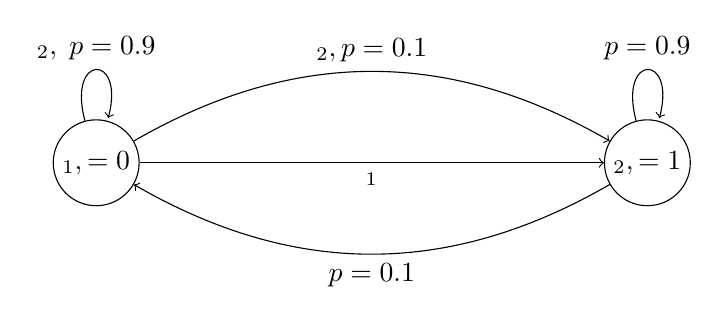
\begin{tikzpicture}[node distance=7cm, auto]
    % Nodes
    \node[draw, circle, inner sep=2pt] (S1) {\(\state_1, \reward=0\)};
    \node[draw, circle, inner sep=2pt, right of=S1] (S2) {\(\state_2, \reward=1\)};
    
    % Edges from S1
    \draw[->, bend left] (S1) to node[midway, above] {\(\action_2, p=0.1\)} (S2);
    \draw[->, right] (S1) to node[midway, below] {\(\action_1\)} (S2);
    \draw[->] (S1) edge[loop above] node {\(\action_2,\;p=0.9\)} (S1);
    
    % Edges from S2
    \draw[->] (S2) edge[loop above] node {\(p=0.9\)} (S2);
    \draw[->, bend left] (S2) to node[midway, below] {\(p=0.1\)} (S1);
\end{tikzpicture}
    \caption{Example MDP}
    \label{fig:vi_vs_pi_example}
\end{figure}
Let the policy in state \(\state_1\) be parametrized by $x$:
\[
x = \policy(\action_1), \quad \text{and hence} \quad \policy(\action_2) = 1-x.
\]
The corresponding Bellman equations for the value functions are:

\[
\begin{aligned}
\Value^\policy(\state_1) &= \gamma \Bigl[ x\,\Value^\policy(\state_2) + (1-x)\Bigl(0.1\,\Value^\policy(\state_2) + 0.9\,\Value^\policy(\state_1)\Bigr)\Bigr], \\
\Value^\policy(\state_2) &= 1 + \gamma \Bigl[0.9\,\Value^\policy(\state_2) + 0.1\,\Value^\policy(\state_1)\Bigr].
\end{aligned}
\]
Thus, substituting \(\gamma = 0.5\):
\[
\Value^\policy(\state_1) = 0.5 \Bigl[(0.9x+0.1)\Value^\policy(\state_2) + 0.9(1-x)\Value^\policy(\state_1)\Bigr].
\]
Rearranging, we obtain
\[
\Value^\policy(\state_1) = \frac{0.5(0.9x+0.1)}{0.55+0.45x}\,\Value^\policy(\state_2).
\]
Now, substitute into the \(\state_2\) equation to obtain:
\[
\Value^\policy(\state_2) = \frac{11+9x}{6+4.5x}, \quad
\Value^\policy(\state_1) = \frac{9x+1}{6+4.5x}.
\]
\textbf{Policy Iteration:} we compute PI iterates starting from a policy $\policy_0$ that chooses \(\action_2\) in \(\state_1\), i.e., \(x=0\). Thus,
\[
\begin{aligned}
\Value^{\policy_0}(\state_1) &= \frac{9\cdot 0 + 1}{6 + 4.5\cdot 0} = \frac{1}{6} \approx 0.16667,\\[1mm]
\Value^{\policy_0}(\state_2) &= \frac{11 + 9\cdot 0}{6 + 4.5\cdot 0} = \frac{11}{6} \approx 1.83333.
\end{aligned}
\]
Using the value function for \(\pi_0\), we compute the action-value functions in \(\state_1\):
\[
\begin{aligned}
\QValue^{\policy_0}(\state_1,\action_1) &= 0 + 0.5\,\Value^{\policy_0}(\state_2) \approx 0.5 \times 1.83333 = 0.91667,\\[1mm]
\QValue^{\policy_0}(\state_1,\action_2) &= 0 + 0.5\Bigl[0.1\,\Value^{\policy_0}(\state_2)+0.9\,\Value^{\policy_0}(\state_1)\Bigr] \\
           &\approx 0.5\Bigl[0.18333 + 0.15\Bigr] \approx 0.16667.
\end{aligned}
\]
Since \(\QValue^{\policy_0}(\state_1,\action_1) > \QValue^{\policy_0}(\state_1,\action_2)\), the improved policy \(\pi_1\) chooses \(\action_1\) (i.e., \(x=1\)). Then,
\[
\begin{aligned}
\Value^{\policy_1}(\state_1) &= \frac{9\cdot 1 + 1}{6 + 4.5\cdot 1} = \frac{10}{10.5} \approx 0.95238,\\[1mm]
\Value^{\policy_1}(\state_2) &= \frac{11 + 9\cdot 1}{6 + 4.5\cdot 1} = \frac{20}{10.5} \approx 1.90476.
\end{aligned}
\]
Policy $\policy_1$ is optimal, therefore PI will halt after one iteration. \\
\textbf{Value Iteration:}
the VI updates are as follows. 
\[
V_{k+1}(\state_1) = \max\Bigl\{ 0.5\,V_k(\state_2),\, 0.5\Bigl[0.1\,V_k(\state_2) + 0.9\,V_k(\state_1)\Bigr] \Bigr\},
\]
\[
V_{k+1}(\state_2) = 1 + 0.5\Bigl[0.9\,V_k(\state_2) + 0.1\,V_k(\state_1)\Bigr].
\]
\begin{figure}[ht]
    \centering
    \includegraphics[width=0.8\linewidth]{figures/vi_vs_pi.png}
    \caption{Comparison between VI and PI for the MDP in Figure \ref{fig:vi_vs_pi_example}. PI starts with a policy $x=0$, and VI is initialized with $V_0(\state_1) = 5, V_0(\state_2) = -1$.}
    \label{fig:vi_vs_pi_plot}
\end{figure}
In Figure \ref{fig:vi_vs_pi_plot} we illustrate the differences between the VI and PI algorithms for this MDP, by inspecting the values obtained during the algorithm runs. First, in the green line, we plot the values of all possible policies in this MDP (by varying $x$ in $[0,1]$). Note that the two policy iteration steps correspond to the two end points on this line. Next, we plot the VI iterates. We color in red the iterates for which the greedy policy (with respect to $V_k$) is optimal, while an orange color indicates otherwise. We make several important observations:
\begin{itemize}
    \item While the values of PI steps correspond to values of actual policies, the VI iterates $V_k$ do not necessarily correspond to any possible value functions (in the example, the VI iterates do not intersect the green line). Recall that we are only guaranteed that VI \textit{converges} to the value of an optimal policy. 
    \item Note that the greedy policy with respect to VI iterate converges to an optimal policy before the VI algorithm converged (in this case, already at $k=2$). Still, PI converges faster.
\end{itemize}
\end{example}
% \section{Variants on Value Iteration and Policy Iteration}

% \subsection{Value Iteration - Gauss Seidel Iteration}
% In the standard value iteration: ${\Value_{n + 1}} =
% T_{}^*({\Value_n})$, the vector ${\Value_n}$ is held fixed while all
% entries of ${\Value_{n + 1}}$ are updated. An alternative is to
% update each element ${\Value_n}(\state)$ of that vector as to
% ${\Value_{n + 1}}(\state)$ as soon as the latter is computed, and
% continue the calculation with the new value. This procedure is
% guaranteed to be ``as good'' as the standard one, in some sense, and
% often speeds up convergence.


% \subsection{Asynchronous Value  Iteration}
% Here, in each iteration ${\Value_n} \Rightarrow {\Value_{n + 1}}$,
% only a subset of the entries of  ${\Value_n}$ (namely, a subset of
% all states) is updated. It can be shown that if each state is
% updated infinitely often, then ${\Value_n} \to {\Value^*}$.
% Asynchronous update can be used to focus the computational effort on
% ``important'' parts of a large-state space.



% \subsection{Modified (a.k.a. Generalized or Optimistic) Policy Iteration}\label{ss:mod_PI}

% This scheme combines policy improvement steps with value iteration
% for policy evaluation. This way the requirement for exact policy
% evaluation (computing  ${\Value^{{\policy _k}}} = {(I - \discount
% {P^{{\policy _k}}})^{ - 1}}{r^{{\policy _k}}}$) is avoided.

% The procedure starts with some initial value vector ${\Value_0}$,
% and iterates as follows:
% \begin{itemize}
%   \item Greedy policy computation:

% Compute ${\policy _k} \in \arg {\max _\policy }T_{}^\policy
% ({\Value_k})$, a greedy policy with respect to ${\Value_k}$.
%   \item Partial fixed-point value iteration:

% Perform ${m_k}$ steps of value iteration, ${\Value_{k + 1}} =
% {(T_\discount ^{{\policy _k}})^{{m_k}}}({\Value_k})$.
% \end{itemize}

% This algorithm guarantees convergence of ${\Value_ k}$ to
% ${\Value^*}$.

%%%%%%%%%%%%%%%%%%%%%%%%%%%%%%%%%%%%%%%%%%


% \begin{leftbar}
% \section{Linear Program}
% \label{chapter-discount:section:LP}

% %[Good idea to add to get them familiar with the notion and notation for the very simple case.]



% %\section{Linear Programming for Finite Horizon}
% In this section we will use linear programming to derive the optimal
% policy for discounted return.
% %
% We will extend the linear programming given in Section
% \ref{C-MDP-FH:sec:LP} from Finite Horizon return to discounted
% return, but the derivation is similar in spirit.
% %
% %[YM: The preliminaries of the Linear Programming should move here
% %from Chapter of discounted return, if we keep this.]
% %
% We will see that both the primal and dual program will play an
% important part in defining the optimal policy. We will fix an
% initial state $\state_0$ and compute the optimal policy for it.

% We will start with the primal linear program, which will compute the
% optimal policy. For each state $\state$ and action $\action$ we will
% have a variable $x(\state,\action)$ that will indicate the
% discounted fraction of time we are at state $\state$ and perform
% action $\action$.

% To better understand what we mean by the ``discounted fraction of
% time'' consider a fixed policy $\policy$ and a trajectory
% $(\state_0, \ldots )$ generated by $\policy$. Define
% $X^\policy(\state,\action)=\sum_\ttime
% \I(\state_\ttime=\state,\action_\ttime=\action)$, which is a random
% variable. We are interested in
% $x^\policy(\state,\action)=\E[X^\policy(\state,\action)]$ which is
% the expected discounted fraction of time policy $\policy$ is in
% state $\state$ and performs action $\action$. The goal of our linear
% program is to compute $x^{\policy^*}$ for the optimal policy
% $\policy^*$.

% Our main constraint will be a flow constraint, stating that the
% discounted fraction of time we reach state $\state$ upper bounds the
% discounted fraction of time we exit it, times the discounted factor.
% Formally, for $\state\in\States$,
% \[
% \I(\state=\state_0)+\sum_{\action} x(\state,\action)\leq \discount
% \sum_{\state',\action'}
% x(\state',\action')\transitionprob(\state|\state'\action').
% \]
% Note that if we sum the inequalities over all states, we have
% \[
% 1+\sum_{\state,\action} x(\state,\action)\leq\discount
% \sum_{\state',\action'} x(\state',\action')\sum_\state
% \transitionprob(\state|\state'\action')=\discount \sum_{\state',\action'}
% x(\state',\action').\]
% %
% which implies that $\sum_{\state,\action} x(\state,\action)\leq
% 1/(1-\discount)$, as we should expect. Namely, in each time we are
% in some state, therefore the sum over states should be $\sum_\ttime
% \discount^\ttime=1/(1-\discount)$.

% The discounted return, which we would like to maximize, is
% $\E[\sum_\ttime
% \discount^\ttime\reward(\state_\ttime,\action_\ttime) ]$. We can
% regroup the sum by state and action and have
% $\sum_{\state,\action}\E[\sum_\ttime
% \discount^\ttime\reward(\state_\ttime,\action_\ttime)\I(\state_\ttime=\state,\action_\ttime=\action)]$,
% which is equivalent to $\sum_{\state,\action}\reward(\state,\action)
% \E[\sum_\ttime
% \discount^\ttime\I(\state_\ttime=\state,\action_\ttime=\action)]$.
% Now our variable are $x(\state,\action)=\E[\sum_\ttime
% \discount^\ttime\I(\state_\ttime=\state,\action_\ttime=\action)]$,
% and the expected return would be
% \[
% \sum_{\state,\action} \reward(\state,\action)x(\state,\action)
% \]


% The resulting linear program is the following.

% \begin{align*}
% \max_{x(\state,\action)}&\;\;\; \sum_{\state,\action}
% \reward(\state,\action)x(\state,\action)\\
% &\mbox{ such that }\\
% %
% &\I(\state=\state_0)+\sum_{\action} x(\state,\action)\leq \discount
% \sum_{\state',\action'} x(\state',\action')\transitionprob(\state|\state'\action')
% &\quad\forall \state \in {\States}, \action\in\Actions,\\
% %
% % &\sum_{\action}
% %x_{\ttime}(\state,\action)=\sum_{\state',\action'}
% %x_{\ttime-1}(\state',\action')p_{\ttime-1}(\state|\state'\action').
% % &\quad\forall
% %\state \in {\States_{\ttime}}, \action\in\Actions,
% %\ttime\in\T\\
% %
% &x(\state,\action) \geq 0  &\quad\forall \state \in {\States},
% \action\in\Actions,
% \\
% %
% %&x_{\ttime}(\state,\action) \leq 1   &\quad\forall \state \in
% %{\States_{\ttime}}, \action\in\Actions,
% %\ttime\in\{0,\ldots,\tHorizon-1\}\\
% %
% &\sum_{\action}x_{0}(\state_0,\action)=1 &\quad\forall \action\in\Actions,\\
% &x_{0}(\state,\action)=0,  &\quad\forall \state \in {\States},
% \state\neq \state_0\\
% \end{align*}

% Given the primal linear program we can derive the dual linear
% program.
% \begin{align*}
% \min_{z(\state)}  \;z_0(\state_0)&\\
% \mbox{ such that }\\
% %
%  z(\state) &\geq
% \reward(\state,\action) + \discount
% \sum_{\state'}z(\state')\transitionprob(\state'|\state,\action) , &\quad\forall
% \state \in {\States},\action\in\Actions, \\ .
% \end{align*}

% One can identify the dual random variables $z(\state)$ with the
% optimal vale function $\Value(\state)$. At the optimal solution of
% the dual linear program one can show that we have
% \begin{align*}
%  z(\state) &= \max_\action \big\{
% \reward(\state,\action) + \discount
% \sum_{\state'}z(\state')p_{\ttime}(\state'|\state,\action) \big\} ,
% &\quad\forall \state \in {\States},
% \end{align*}
% which are the familiar Bellman optimality equations.

% %
% %
% %\begin{proposition}
% %The solution $v_\ttime(\state)$ of the linear program is the optimal
% %value function $\Value_{ttime}(\state)$.
% %\end{proposition}
% %
% %\begin{proof}
% %Let $v_\ttime(\state)$ be the solution of the linear program. We
% %will show by back ward induction that the values $v_\ttime(\state)$
% %are identical to $\Value_\ttime(\state)$ of the Finite-horizon
% %Dynamic Programming (Algorithm \ref{Alg:FHDP-DDP}), i.e,
% %$v_\ttime(\state)=\Value_\ttime(\state)$.
% %
% %At $\ttime=\tHorizon$ it holds by the initializations in both cases.
% %Consider $\ttime$ and assume that the inductive hypothesis holds for
% %$\ttime+1$. This implies that for every action $\action\in\Actions$
% %nd state $\state\in\States$, we have
% %\[{{\reward_{\ttime}}(\state,\action) + \Value_{\ttime +
% %1}^{}({f_{\ttime}}(\state,\action))}=
% %{{\reward_{\ttime}}(\state,\action) + v_{\ttime +
% %1}^{}({f_{\ttime}}(\state,\action))} .\]
% %Therefore we have
% %$v_\ttime(\state) \geq \Value_\ttime(\state)$. Since we are
% %minimizing over $v_\ttime(\state)$, we have $v_\ttime(\state) \geq
% %\Value_\ttime(\state)$.
% %\end{proof}

% \end{leftbar}

% \section{Exercises}
% \subsection{Modified Policy Iteration:}
In this question we will analyze the Modified Policy Iteration (MPI) algorithm~\ref{alg:MPI}. 
% Denote the fixed-policy and optimal Bellman operators as $T^\pi$ and $T$, respectively. 
\begin{center}
\begin{minipage}{1.1\textwidth}
\begin{algorithm}[H]
	\caption{MPI}
	\label{alg:MPI}
	\begin{algorithmic}
		\STATE {\bfseries Initialize:} $m \in \mathbb{N},~\Value_0 \in \mathbb{R}^{|\States|}$
		\WHILE{some stopping criterion}
			\FOR{ $\state\in \States$}
				\STATE $\policy_{k+1}(\state)\in \arg\max_{\action} \reward(\state,\action) + \gamma \sum_{\state'}\transitionprob(\state' | \state,\action)\Value_k(\state').$
			\ENDFOR
			\FOR{$\state\in \States$}
				\STATE $\Value_{k+1}(\state)= \sum_{\ttime=0}^{m-1}\sum_{\state'} \gamma^\ttime \transitionprob(\state_\ttime=\state' | \state_0=\state,\policy_{k+1}) \reward(\state',\policy_{k+1}(\state')) +\gamma^m \sum_{\state''}\transitionprob(\state_m=\state'' | \state_0=\state, \policy_{k+1})\Value_{k}(\state'').$
			\ENDFOR
		\ENDWHILE
		\STATE {\bfseries Return $\policy,\Value$}
	\end{algorithmic}
\end{algorithm}
\end{minipage}
\end{center}

\begin{itemize}
\item [a.] In a vector notation, MPI performs the following two steps of policy and value update,
\begin{enumerate}
\item $\policy_{k+1} \in \{\policy': T^{\policy'}\Value_k=T \Value_k \}$.
\item $\Value_{k+1} =\left(T^{\policy_{k+1}}\right)^m \Value_{k}$.
\end{enumerate}
Prove the two algorithms are equivalent.
\item [b.] Describe which algorithms are obtained when $m=1,m\to\infty$? 
\end{itemize}

In the rest of the question we will analyze the convergence of Modified Policy Iteration.
\begin{itemize}
\item [c.] Assume that $T \Value_0\geq \Value_0$. Prove the following (component-wise) inequalities $$\Value_0\leq T^{\policy_1} \Value_0 \leq \cdot\cdot\cdot \leq (T^{\policy_1})^m \Value_0\leq (T^{\policy_1})^{m+1} \Value_0 \leq \cdot \cdot \cdot \leq \Value^{\policy_1} \leq \Value^*.$$
Do the inequalities hold without the assumption? prove or give a counter-example.
\item [d.] Assume that $T \Value_0\geq \Value_0$. Prove that for any $k$, $T \Value_k\geq \Value_k$ (component-wise) and thus $$\Value_{k-1}\leq T^{\policy_k}\Value_{k-1} \leq \cdot\cdot\cdot \leq (T^{\policy_k})^m \Value_{k-1} \leq (T^{\policy_k})^{m+1} \Value_{k-1}\leq \cdot \cdot \cdot \leq \Value_{\policy_{k}}\leq \Value_*$$ for any $k$.
Hint: use induction, and the update rule of MPI, $\Value_k=(T^{\policy_k})^m \Value_{k-1}$.
\item [e.] Prove $\norm{\Value_*-\Value_k}_\infty \leq \gamma \norm{\Value_*-\Value_{k-1}}_\infty$. Hint: prove $0 \leq \Value_*-\Value_k\leq T\Value_* - T\Value_{k-1}$ and then take the max-norm.
\end{itemize}
% \subsection{MDP with a reward-ratio objective:}
Consider an MDP $\mathcal{M}$ with finite state space $\mathcal{S}$ and finite actions space $\mathcal{A}$, transitions $P(s'|s,a)$, discount factor $\gamma\in (0,1)$, a \textbf{fixed} initial state $s_{init}$, and \textbf{two} reward functions: $r_1(s)$ and $r_2(s)$. In this question we will consider objectives that are a function of both $r_1$ and $r_2$.

For a Markov policy $\pi$, we denote the discounted returns $J_1^\pi$ and $J_2^\pi$ as:
\begin{equation*}
\begin{split}
    J_1^\pi &= \mathbb{E}^\pi \left[\left. \sum_{t=0}^\infty \gamma^t r_1(s_t)\right|s_0 = s_{init}\right], \\
    J_2^\pi &= \mathbb{E}^\pi \left[ \left.\sum_{t=0}^\infty \gamma^t r_2(s_t)\right|s_0 = s_{init}\right].
\end{split}
\end{equation*}

Note that the initial state is fixed, and that $J_1^\pi, J_2^\pi$ denote scalar returns and not value functions.

Let $f(x,y)$ be some function of two variables. For some policy $\pi$ we denote $J^\pi = f(J_1^\pi, J_2^\pi).$ We wish to find a policy $\pi^*$ that maximizes $J^\pi$:
\begin{equation*}
    J^* = \max_{\pi} J^\pi, \quad \pi^* \in \argmax_{\pi} J^\pi.
\end{equation*}

\begin{itemize}
    \item[a.] For $f(x,y)=\alpha x +\beta y$, propose a standard MDP with a single reward $\hat{r}$ such that it's optimal policy is $\pi^*$. Explain.
\end{itemize}

For the rest of this question, we consider the function $f(x,y) = \frac{x}{y}$. Furthermore, we assume the following bounds on the rewards: $0<r_{min}\leq r_1(s) < r_2(s) \leq r_{max}$, for all $s\in\mathcal{S}$. 

\begin{itemize}
    \item[b.] Can the standard MDP solution approaches (value iteration, policy iteration) be used to find $\pi^*$ in this case? Explain (no need to prove formally).
\end{itemize}

For some $\rho \in [0,1]$, consider a standard MDP $\mathcal{M}_{\rho}$ with the same $\mathcal{S},\mathcal{A},P,\gamma$ as $\mathcal{M}$ and reward $\hat{r}(s) = r_1(s) - \rho r_2(s).$ Denote the discounted reward for a policy $\pi$ in $\mathcal{M}_{\rho}$ as $J_{\rho}^\pi = \mathbb{E}^\pi \left[ \sum_{t=0}^\infty \gamma^t \hat{r}(s_t)|s_0 = s_{init}\right]$.

\begin{itemize}
    \item[c.] Assume that for some policy $\pi$, we have that $J_{\rho}^\pi = 0$. What is $J^\pi$?
    \item[d.] Let $\pi_\rho^*$ be an optimal policy in $\mathcal{M}_{\rho}$, that also satisfies  $J_{\rho}^{\pi_\rho^*} = 0$. Show that $\pi_\rho^*$ is optimal also in $\mathcal{M}$.
    
    Hint: assume that for some $\pi'$, $J^{\pi'} > \rho$, and show a contradiction.
    
    \item[e.] Show that for $\rho=0$, $J_{\rho}^\pi > 0$ for any $\pi$.
    \item[f.] Show that for $\rho=1$, $J_{\rho}^\pi < 0$ for any $\pi$.
    \item[g.] Let $J_{\rho}^*$ denote the optimal value in $\mathcal{M}_{\rho}$. Show that $J_{\rho}^*$ is monotonically decreasing in $\rho$.
    
    Hint: start by showing monotonicity for a fixed policy.
    \item[h.] Based on (d-g), propose an approach for finding the optimal policy $\pi^*$. Technically, you can assume that $J_{\rho}^*$ is continuous in $\rho$, and you can invoke any standard MDP solver in your solution.
    
\end{itemize}
% \subsection{Purchasing with a deadline}
Consider the following scenario: as the purchasing manager of a factory, you have $T$ days to buy a certain material that is required for the production process. At the beginning of each day $k$, you observe a price offer for the material $x_k \sim \mathit{Uniform}[a,b]$, drawn independently of the prices at other days. You may decide to either buy the material at the price $x_k$ (and then the scenario ends), or wait for the next day. If a purchase hasn't been made by day $T$, the product has to be purchased at the last price $x_T$.

The goal is to decide when to buy the material, such that its price (in expectation) is lowest.

1. Explain intuitively, why the optimal decision whether to buy at some price $x$ may be different at different days.

We formulate the problem as a finite horizon MDP as follows. The state space at time $k$ is $x_k\in [a,b]$. The action space is binary $a_k \in \{buy,hold\}$. Once a $buy$ action is executed at state $x_k$, an immediate cost of $x_k$ is incurred, and the state transitions to a terminal state $x^*$ with zero cost. Otherwise, if a   $hold$ action is executed, no cost is incurred, and the state transitions to $x_{k+1} \sim \mathit{Uniform}[a,b]$. At time $k=T$, the only available action is $buy$. Also, once the terminal state is reached, the state no longer changes, and no cost is further incurred.

2. Define the optimal value function $V_k(x) \doteq \inf_\pi \mathbb{E}^\pi \left[ \sum_{t=k}^{T} c(x_t,\pi(x_t)) | x_k = x\right]$. Note that by definition $V_k(x^*)=0$ for all $k$.

%\quad a. What is $V_k(x^*)$?

\quad a. What is $V_T(x)$?

\quad b. Write a recursive equation for $V_k(x)$ as a function of  $V_{k+1}(x)$.

3. For $a=0,b=1$, draw the value functions $V_T(x)$, $V_{T-1}(x)$, and $V_{T-2}(x)$.

4. Prove that the optimal policy is a threshold policy, given by
\begin{equation*}
\left\{
  \begin{array}{ll}
    buy, & \text{if } x_k \leq \alpha_k \\
    hold, & \text{if } x_k > \alpha_k.
  \end{array}
\right.
\end{equation*}

\quad Write a recursive equation for $\alpha_k$.

\vspace{20pt}
From now on, we consider a scenario where there is correlation between the prices at different days. Specifically:
\begin{equation*}
    x_{k+1} = \lambda x_k + \epsilon_k,
\end{equation*}
where $0 \leq \lambda < 1$ is a known constant, and $\{\epsilon_k\} \in [0,b]$ are i.i.d. random variables with a known distribution $p(\epsilon)$. Let $\bar{\epsilon} = \mathbb{E} [\epsilon_k ]$, and assume that $\bar{\epsilon} > 0$. The state space in this case is $x_k\in \mathbb{R}$.

5. Write a recursive equation for the value function $V_k(x)$ for this scenario.

\vspace{10pt}

We will now show that in the correlated case as well, the optimal policy is a threshold policy. We will do this in several steps.

A function $f(x)$ is said to be \emph{concave} if, for any $x,y$ and $\beta \in [0,1]$, it holds that $f(\beta x + (1-\beta) y) \geq  \beta f(x) + (1-\beta) f(y)$.

6. Prove that if $f(x)$ is concave, then $\mathbb{E} [f(\lambda x + \epsilon_k)]$ is also concave.

7. Prove that for all $1 \leq k \leq T$, the value function $V_k(x)$ is concave.

\quad \textbf{Hint}: you may use the following fact: the minimum of two concave functions is concave.

%A function $f(x)$ is said to be \emph{increasing} if, for any $x<y$ it holds that $f(x) < f(y)$.

8. * Prove that the optimal policy is again a threshold policy.

\quad \textbf{Hint}: You may first prove that for all $1 \leq k \leq T$, $V_k(x)$ is increasing, and positive for $x\geq 0$. 

\section{Further Remarks on Policy Iteration}
\label{disc:bib}

% The value iteration method dates back  to Bellman \cite{Bellman:DynamicProgramming}.
% The computational complexity analysis of value iteration first explicitly appeared in \cite{LittmanDK95}.
%
% The work of Blackwell \cite{blackwell1965discounted} introduces the contracting operators and the fixed point for the analysis of MDPs.

Policy iteration originated in the work of Howard \cite{Howard1960}.
There has been significant interest in bounding the number of iteration of policy iterations, with a dependency only on the number of states and actions. A simple upper bound is the number of policies, $|\Actions|^{|\States|}$, since each policy is selected at most once.
The work of \cite{MelekopoglouC94} shows a lower bound of $\Omega(2^{|\States|/2})$ for a special class of policy iteration, where only a single state of all improving states is updated and two actions.
The work of \cite{MansourS99} shows that if the policy iteration updates with all the improving states (as it is define here) then the number of iterations is at most $O(|\Actions|^{|\States|}/|\States|)$.
The work of \cite{Fearnley10} shows a $n$-state and $\Theta(n)$ action MDP for which the policy iteration requires $\Omega(2^{n/7})$ iterations for the average cost return, and \cite{HollandersDJ12} for the discounted return. Surprisingly, for a constant discount factor, the bound on the number of iterations is polynomial \cite{Ye11,HansenMZ13}.




%The work of \cite{d1963probabilistic} was the first to formalize a Linear Programming for the discounted return, and \cite{manne1960linear} for the average cost.
%There are works that use a linear programming approach to derive strongly polynomial algorithms. Specifically, for deterministic MDPs we have polynomial time algorithms which are based on linear programming \cite{MadaniTZ10,PostY13}.